\documentclass{article}
\usepackage{graphics} 
\usepackage{hyperref}
\usepackage{fixltx2e}
\usepackage{amssymb}
\usepackage{tikz}

\author{Kevin Zollicoffer}
\title{Regression\\Lesson 3a}
\date{10/28/2013}

% no indents
\setlength\parindent{0pt}

\usepackage{Sweave}
\begin{document}
\maketitle
%\tableofcontents
\Sconcordance{concordance:Assignment3a.tex:Assignment3a.Rnw:%
1 14 1 1 0 14 1 1 2 1 0 2 1 3 0 2 2 1 0 4 1 4 0 2 2 1 0 1 1 22 0 1 2 2 %
1 1 2 24 0 1 2 12 1 1 2 1 0 2 1 4 0 1 2 1 1 1 2 1 0 2 1 3 0 1 2 2 1 1 2 %
1 0 1 1 21 0 1 2 1 1 21 0 1 2 3 1 22 0 1 2 2 1 1 2 1 0 1 1 22 0 1 2 8 1 %
1 2 1 0 1 1 5 0 1 3 1 1}


\section*{Introduction}
Regression assignment 3a using R
\\
\\
The complete source for this assigment is available on Github:
\\
\\
\url{https://github.com/zollie/PASS-Regression-Assignment3a}

\section*{Problem 4.1}
\begin{Schunk}
\begin{Sinput}
> nyj <- read.csv("~/R/PASS/Regression/Assignment3a/nyjuice.csv")
> nyj$DaySq <- nyj$Day**2
> attach(nyj)
\end{Sinput}
\end{Schunk}
\subsection*{a}
\begin{Schunk}
\begin{Sinput}
> plot(nyj$Day, nyj$Cases)
> model <- lm(Cases ~ Day + DaySq)
> newX <- seq(min(nyj$Day), max(nyj$Day), length=nrow(nyj))
> newXsq <- newX**2
> lines(newX, predict(model, newdata=data.frame(Day=newX, Xsq=newXsq)))
\end{Sinput}
\end{Schunk}
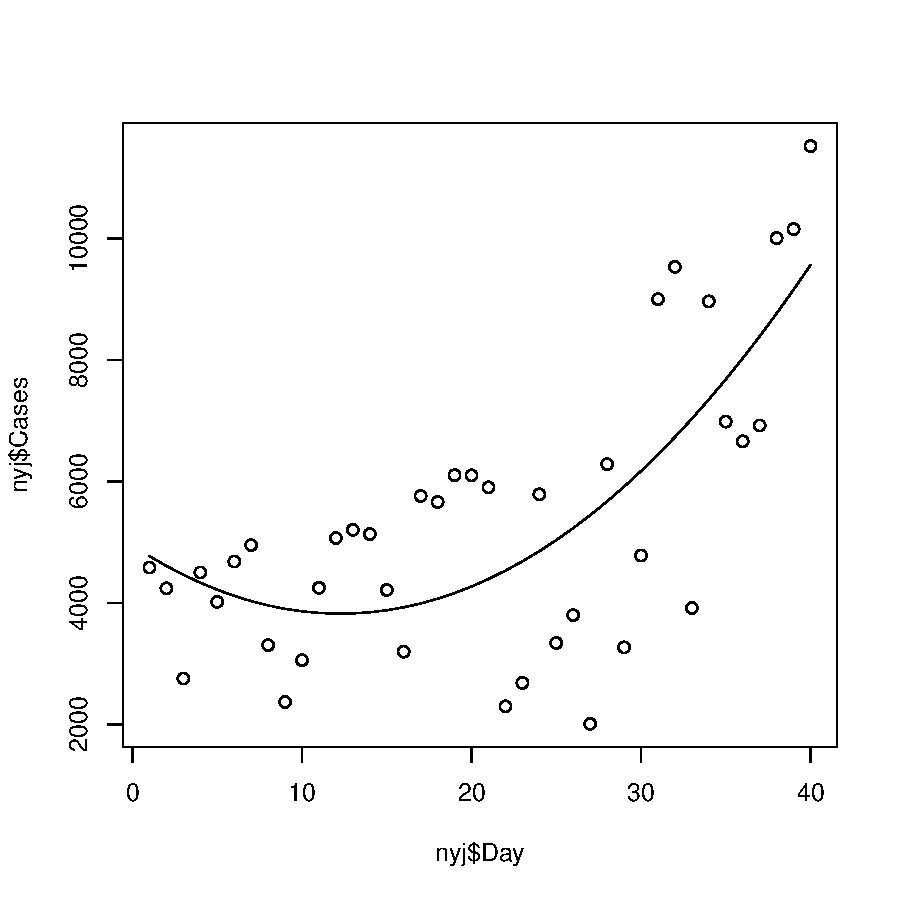
\includegraphics{Assignment3a-002}
\subsection*{b}
\begin{Schunk}
\begin{Sinput}
> model_simp <- lm(Cases ~ Day)
> summary(model_simp)
\end{Sinput}
\begin{Soutput}
Call:
lm(formula = Cases ~ Day)

Residuals:
    Min      1Q  Median      3Q     Max 
-4115.0 -1118.1   305.4  1152.6  3799.6 

Coefficients:
            Estimate Std. Error t value Pr(>|t|)    
(Intercept)   2802.4      604.7   4.634 4.13e-05 ***
Day            123.0       25.7   4.783 2.61e-05 ***
---
Signif. codes:  0 ‘***’ 0.001 ‘**’ 0.01 ‘*’ 0.05 ‘.’ 0.1 ‘ ’ 1

Residual standard error: 1877 on 38 degrees of freedom
Multiple R-squared:  0.3758,	Adjusted R-squared:  0.3594 
F-statistic: 22.88 on 1 and 38 DF,  p-value: 2.606e-05
\end{Soutput}
\end{Schunk}

$\hat{Y}=2802.4+Day123$
\subsection*{c}
\begin{Schunk}
\begin{Sinput}
> summary(model)
\end{Sinput}
\begin{Soutput}
Call:
lm(formula = Cases ~ Day + DaySq)

Residuals:
    Min      1Q  Median      3Q     Max 
-3435.9 -1401.3   251.3  1310.1  2801.7 

Coefficients:
            Estimate Std. Error t value Pr(>|t|)    
(Intercept) 4944.221    829.601   5.960 7.12e-07 ***
Day         -183.029     93.319  -1.961  0.05740 .  
DaySq          7.463      2.207   3.381  0.00172 ** 
---
Signif. codes:  0 ‘***’ 0.001 ‘**’ 0.01 ‘*’ 0.05 ‘.’ 0.1 ‘ ’ 1

Residual standard error: 1662 on 37 degrees of freedom
Multiple R-squared:  0.5232,	Adjusted R-squared:  0.4974 
F-statistic:  20.3 on 2 and 37 DF,  p-value: 1.122e-06
\end{Soutput}
\end{Schunk}

$\hat{Y}=4944.221-Day183.029+DaySq7.463$

\subsection*{c}
$H_0: DaySq=0$
\\
$H_a: DaySq\neq0$
\\\\
The p-value for DaySq is 0.00172 < .05 therefore, we reject the $H_0$ as it appears there is statistical eveidence to support $H_a$

\section*{Problem 4.3}
The data are scatter plotted first for visual inspection. 

\begin{Schunk}
\begin{Sinput}
> options(scipen=999)
> elec <- read.csv("~/R/PASS/Regression/Assignment3a/internet.csv")
> plot(elec$Gdp, elec$Int)
\end{Sinput}
\end{Schunk}
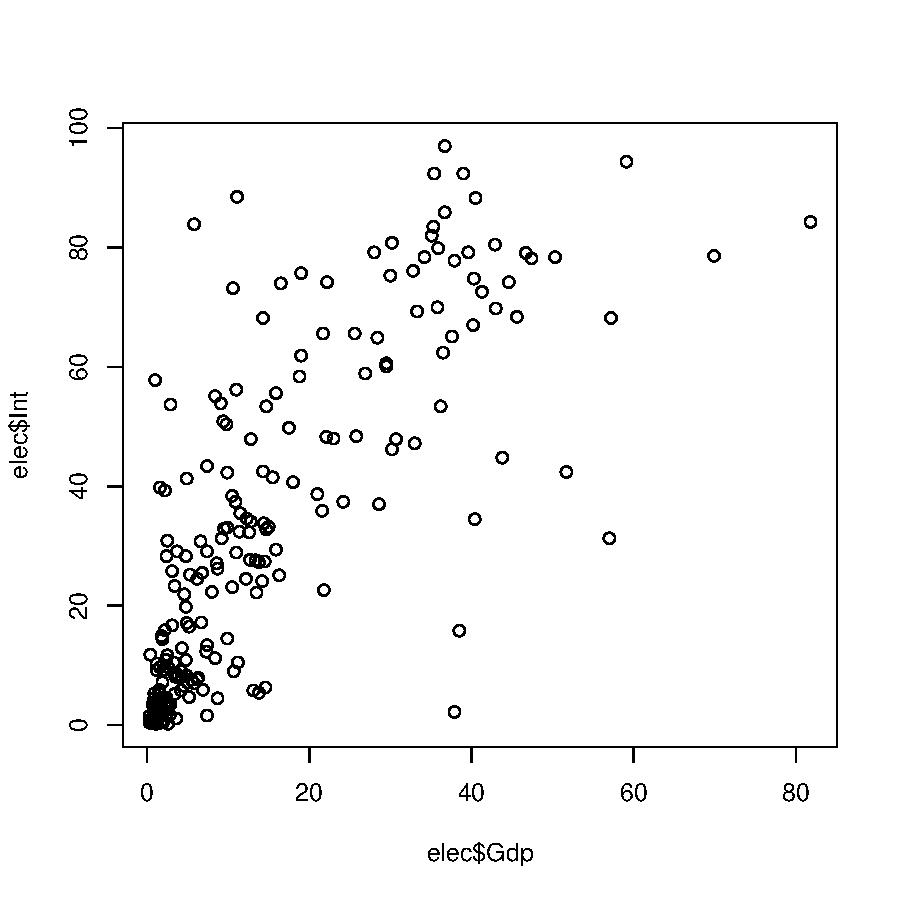
\includegraphics{Assignment3a-005}

This data is highly skewed to the right. We drop the two extreme outliers from the data. 
\begin{Schunk}
\begin{Sinput}
> max2 <- order(elec$Gdp,decreasing=T)[1:2]
> elec2 <- elec[-max2,]
> attach(elec2)
\end{Sinput}
\end{Schunk}

Next, 3 models are examaned.

\begin{Schunk}
\begin{Sinput}
> model.A <- lm(Int ~ Gdp)
> summary(model.A)
\end{Sinput}
\begin{Soutput}
Call:
lm(formula = Int ~ Gdp)

Residuals:
    Min      1Q  Median      3Q     Max 
-64.353 -11.079  -3.247   9.184  64.137 

Coefficients:
            Estimate Std. Error t value             Pr(>|t|)    
(Intercept) 11.30877    1.72759   6.546       0.000000000453 ***
Gdp          1.45763    0.08495  17.158 < 0.0000000000000002 ***
---
Signif. codes:  0 ‘***’ 0.001 ‘**’ 0.01 ‘*’ 0.05 ‘.’ 0.1 ‘ ’ 1

Residual standard error: 17.85 on 208 degrees of freedom
Multiple R-squared:  0.586,	Adjusted R-squared:  0.584 
F-statistic: 294.4 on 1 and 208 DF,  p-value: < 0.00000000000000022
\end{Soutput}
\begin{Sinput}
> model.B <- lm(log(Int) ~ log(Gdp))
> summary(model.B)
\end{Sinput}
\begin{Soutput}
Call:
lm(formula = log(Int) ~ log(Gdp))

Residuals:
    Min      1Q  Median      3Q     Max 
-3.4847 -0.3929  0.0805  0.4740  3.0290 

Coefficients:
            Estimate Std. Error t value             Pr(>|t|)    
(Intercept)  1.02800    0.11623   8.845 0.000000000000000397 ***
log(Gdp)     0.88670    0.04891  18.130 < 0.0000000000000002 ***
---
Signif. codes:  0 ‘***’ 0.001 ‘**’ 0.01 ‘*’ 0.05 ‘.’ 0.1 ‘ ’ 1

Residual standard error: 0.9078 on 208 degrees of freedom
Multiple R-squared:  0.6125,	Adjusted R-squared:  0.6106 
F-statistic: 328.7 on 1 and 208 DF,  p-value: < 0.00000000000000022
\end{Soutput}
\begin{Sinput}
> elec2$Gdp_C <- elec2$Gdp**.5
> elec2$Int_C <- elec2$Int**.5
> model.C <- lm(Int_C ~ Gdp_C, data=elec2)
> summary(model.C)                     
\end{Sinput}
\begin{Soutput}
Call:
lm(formula = Int_C ~ Gdp_C, data = elec2)

Residuals:
    Min      1Q  Median      3Q     Max 
-6.7722 -1.0818 -0.0734  0.9538  5.1862 

Coefficients:
            Estimate Std. Error t value             Pr(>|t|)    
(Intercept)  1.28408    0.22632   5.674         0.0000000464 ***
Gdp_C        1.13240    0.05993  18.896 < 0.0000000000000002 ***
---
Signif. codes:  0 ‘***’ 0.001 ‘**’ 0.01 ‘*’ 0.05 ‘.’ 0.1 ‘ ’ 1

Residual standard error: 1.629 on 208 degrees of freedom
Multiple R-squared:  0.6319,	Adjusted R-squared:  0.6301 
F-statistic: 357.1 on 1 and 208 DF,  p-value: < 0.00000000000000022
\end{Soutput}
\end{Schunk}

The $log_e$ transformations had the lowest standard error, however the power transform had the highest $R^2$. A forth model was tried thart takes the power of .5 for the response, and the log of the predictor, Gdp

\begin{Schunk}
\begin{Sinput}
> model.D <- lm(Int_C ~ log(Gdp), data=elec2)
> summary(model.D)
\end{Sinput}
\begin{Soutput}
Call:
lm(formula = Int_C ~ log(Gdp), data = elec2)

Residuals:
    Min      1Q  Median      3Q     Max 
-6.2480 -0.9576  0.0962  1.0249  5.9594 

Coefficients:
            Estimate Std. Error t value             Pr(>|t|)    
(Intercept)  1.64325    0.20483   8.022   0.0000000000000746 ***
log(Gdp)     1.67484    0.08619  19.432 < 0.0000000000000002 ***
---
Signif. codes:  0 ‘***’ 0.001 ‘**’ 0.01 ‘*’ 0.05 ‘.’ 0.1 ‘ ’ 1

Residual standard error: 1.6 on 208 degrees of freedom
Multiple R-squared:  0.6448,	Adjusted R-squared:  0.6431 
F-statistic: 377.6 on 1 and 208 DF,  p-value: < 0.00000000000000022
\end{Soutput}
\end{Schunk}

This model has the highest $R^2$, although it may be more troublesome to interpret.

\subsection*{Conclusion}
In this case I would choose model.B of the 4 evaluated due to it's ease of interpretation and relatively high $R^2$ and low standard error compared to the other 3 models. 

\subsection*{Boxcox}
I attempted touse boxcox, but was unsure how to interret it so left it out of the above. 

\begin{Schunk}
\begin{Sinput}
> library(MASS)
> boxcox(model, plotit=TRUE)
> 
\end{Sinput}
\end{Schunk}
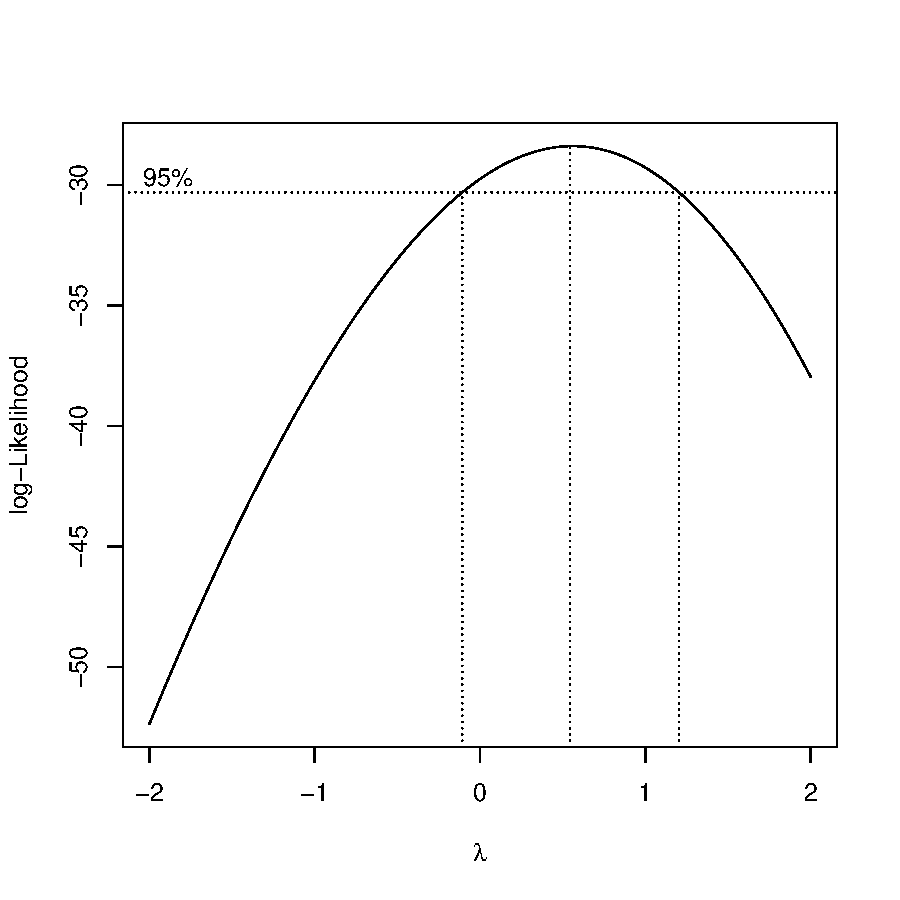
\includegraphics{Assignment3a-009}

\end{document}
